Avant d'établir les liens entre les bases de données, il est essentiel de préparer correctement ces bases. Cela inclut la vérification de la qualité et de la pérennité des données, ainsi que la planification précise de l'insertion des liens dans les fichiers \index{XML}XML et des données ou métadonnées à associer.


\section{Vérification de la qualité des données et de leur pérennité}
Je me suis principalement chargé de la vérification de la qualité des données et de la pérennité de ThEMA, car je n'ai pas eu de tâches similaires du côté de SourcEncyMe.

\

J'ai d'abord rédigé une documentation détaillée sur le fonctionnement et l'installation locale de la base de données. Ce travail, présenté dans les annexes A et B, est crucial pour éviter l'abandon des bases de données lorsque les chercheurs responsables prennent leur retraite. La disparition éventuelle de la base compromettrait la valeur des liens créés. Ce point est d'autant plus pertinent avec le départ prochain à la retraite de \index{Marie-Anne Polo de Beaulieu}Marie-Anne Polo de Beaulieu, directrice scientifique du projet. Il est impératif que cette documentation facilite le transfert de connaissances aux futurs chercheurs ou ingénieurs d'études qui reprendront ThEMA. Actuellement, Jean-Paul Rehr, le créateur de la base, en assure seul la gestion. Il est donc essentiel que ses connaissances soient préservées.

J'ai également résolu un problème lié à l'affichage des \textit{exempla}. Initialement, les \textit{exempla} n'étaient pas classés selon l'ordre du recueil, mais étaient triés en fonction du numéro du fichier XML. Par exemple, un \textit{exemplum} numéroté 10 pourrait apparaître avant un \textit{exemplum} 5.2 si ce dernier avait été ajouté ultérieurement, car son fichier \index{XML}XML avait été généré plus tard. De plus, des incohérences liées aux différentes méthodes d'indexation utilisées par les chercheurs ont été identifiées : certains \textit{exempla} étaient classés avec des notations variées telles que 1.b; 1b; 1, 5, 6. Cette diversité de formats empêchait un classement croissant uniforme. La réorganisation était donc nécessaire pour garantir que les utilisateurs puissent retrouver facilement les \textit{exempla} recherchés. Sans cette réorganisation, les liens vers SourcEncyMe risquaient de devenir moins accessibles. \\

\begin{figure}[H]
	\centering
	\fbox{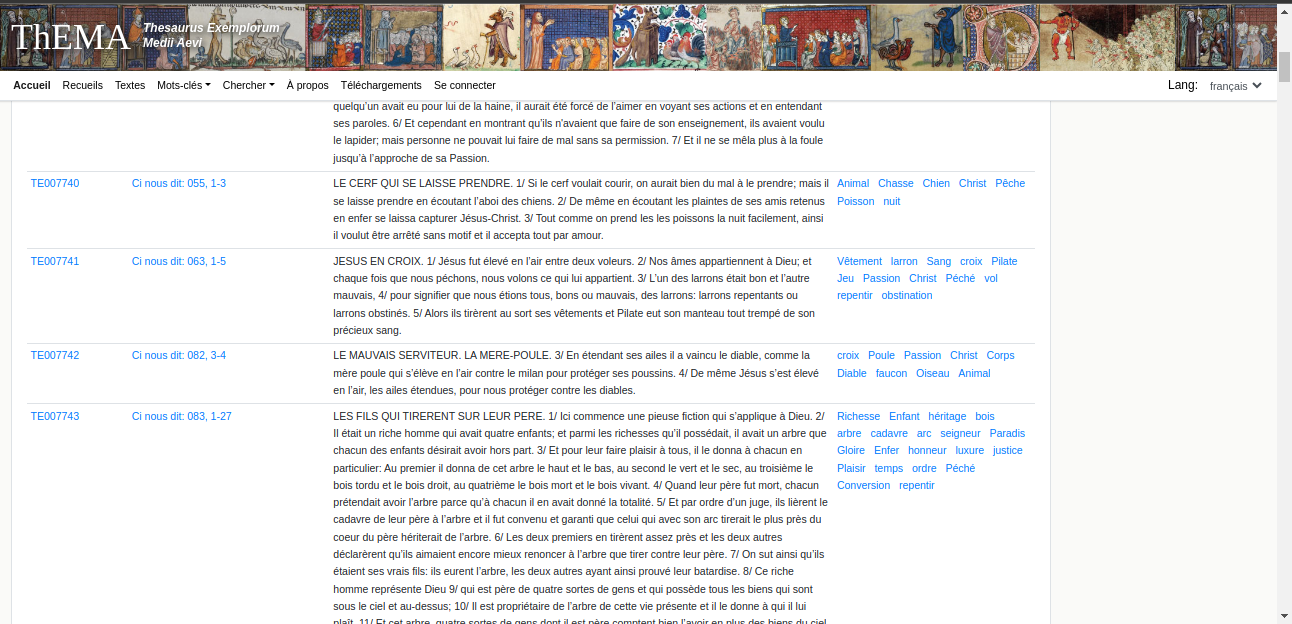
\includegraphics[width=0.8\linewidth]{images/recitsmalclasses.png}}
	\caption{Récits exemplaires mal classés}
\end{figure}

Pour résoudre ce problème, j'ai d'abord développé un code en \index{Python}Python (annexe C). Ce code extrait les numéros des \index{Récits exemplaires}récits exemplaires et convertit les lettres présentes dans la numérotation en chiffres. Cependant, cette méthode a présenté des inconvénients : elle nécessitait de modifier de nombreux types de numérotations et de réintégrer les fichiers \index{XML}XML modifiés dans la base, alors que seulement 30 \% des récits étaient mal classés.

Une approche plus simple a donc été développée pour identifier uniquement les recueils présentant des erreurs de classement et les corriger sans tenter d'uniformiser les numéros des récits. De plus, ce second code a été écrit en \index{XQuery}XQuery (annexe D) afin de s'intégrer directement dans la base de données. Ainsi, en cas de nouvelles erreurs d'indexation, elles seront automatiquement traitées, éliminant la nécessité de relancer le code \index{Python}Python et de réintégrer les données dans la base.


\section{Identifications des liens entre les bases de données}
J'ai identifié des similitudes entre les deux bases de données, tant au niveau des données que des métadonnées. Pour les données, c’est-à-dire les éléments bruts susceptibles de fournir des informations (ici, tu texte), les types de connexions possibles sont les suivants : \\

\begin{itemize}
	\item Quand un \textit{exemplum} d'un recueil de récits exemplaires utilise un morceau d'une \index{Encyclopédies}encyclopédie.
	\item Quand un \textit{exemplum} est repéré dans une encyclopédie et qu'un recueil d'\textit{exempla} contient un \textit{exemplum} similaire ou si on le retrouve dans la classification de l'\textit{Index exemplorum} de Frederic Tubach.
	\item Quand un \textit{exemplum} est identifié dans une encyclopédie et qu'il est indexé dans ThEMA.
\end{itemize}

\

Pour ce qui est des métadonnées, qui fournissent des informations sur d'autres données, voici les éléments pouvant être connectés : \\

\begin{itemize} 
	\item Les \index{Mementos}mementos (fiches de présentation des auteurs ou des œuvres) des deux bases de données et leur contenu respectif peuvent être connectés : \\
	
	\begin{figure}[H]
		\centering
		\fbox{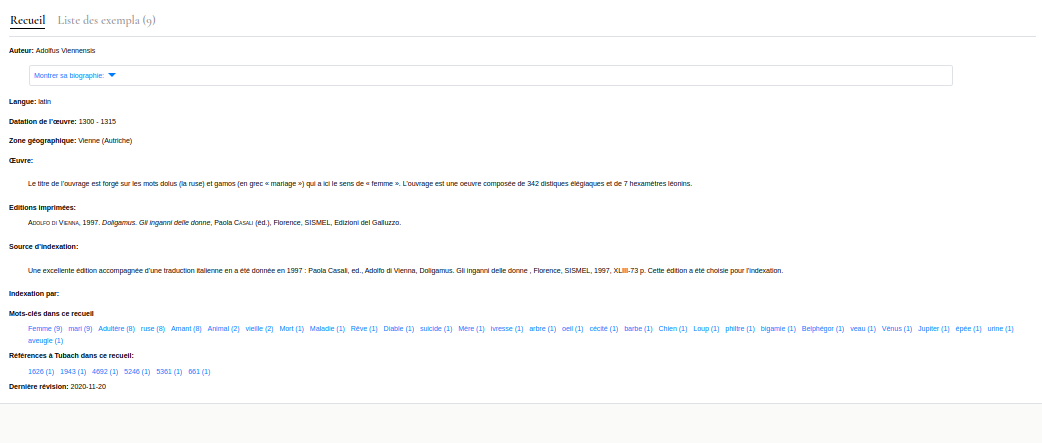
\includegraphics[width=0.8\linewidth]{images/mementothema.png}}
		\caption{Memento dans ThEMA}
	\end{figure}
	
	\begin{figure}[H]
		\centering
		\fbox{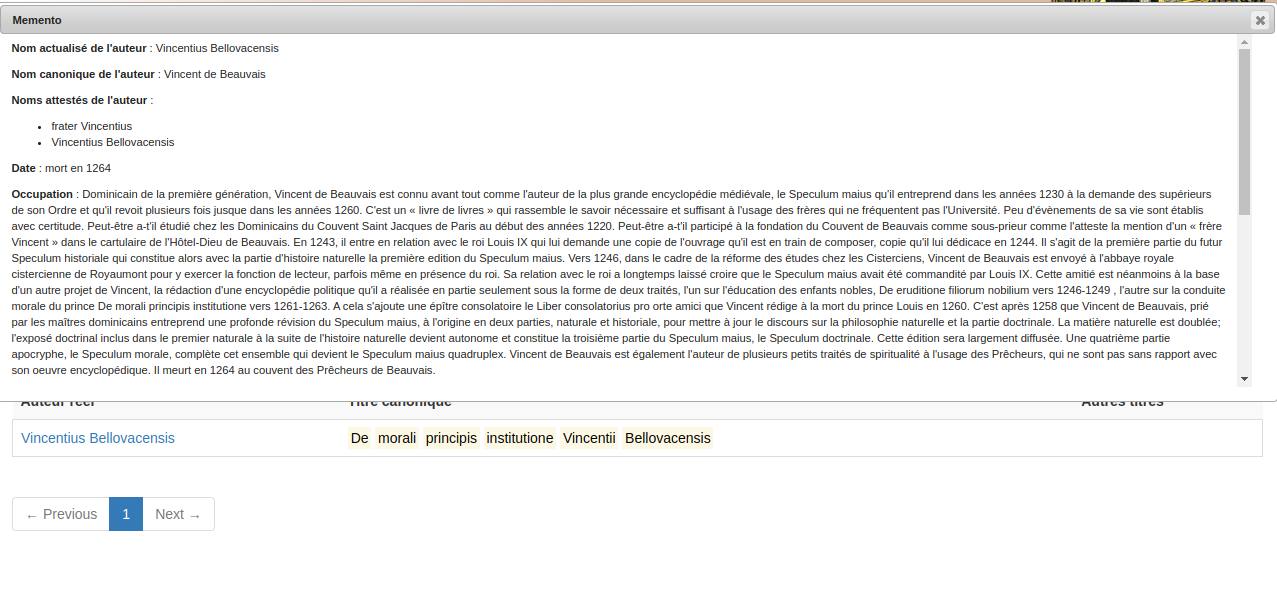
\includegraphics[width=0.8\linewidth]{images/mementosourcencyme.png}}
		\caption{Memento dans SourcEncyMe}
	\end{figure}
	
	\item Les sources des \index{Récits exemplaires}récits exemplaires mentionnées lors de l'indexation sur ThEMA peuvent être connectées aux \index{Mementos}mementos, comme illustré avec Cicéron : \\

	\begin{figure}[H]
		\centering
		\fbox{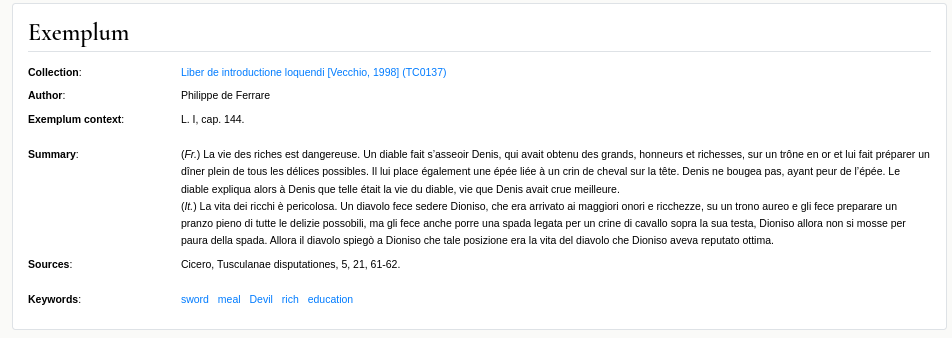
\includegraphics[width=0.8\linewidth]{images/sourcethemacicero.png}}
		\caption{Récit exemplaire utilisant un texte de Cicéron}
	\end{figure}

	\begin{figure}[H]
		\centering
		\fbox{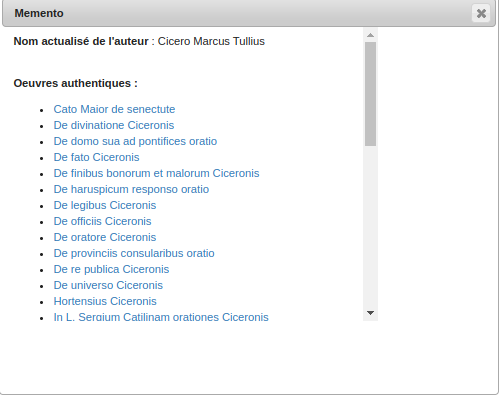
\includegraphics[width=0.6\linewidth]{images/mementociero.png}}
		\caption{Memento de Cicéron}
	\end{figure}
	
	\item Les noms de lieux, de personnes et les thématiques présents dans les mots-clés de ThEMA peuvent être reliés aux textes de SourcEncyMe, comme le montre l'exemple avec Jérusalem : \\
	
	\begin{figure}[H]
		\centering
		\fbox{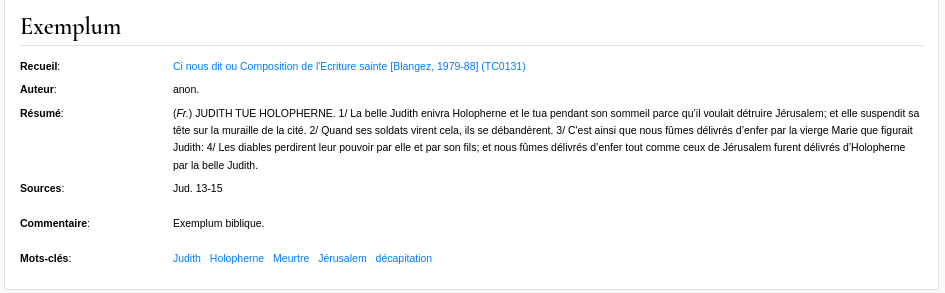
\includegraphics[width=0.8\linewidth]{images/jerusalemthema.png}}
		\caption{Mention de Jérusalem dans ThEMA}
	\end{figure}
	
	\begin{figure}[H]
		\centering
		\fbox{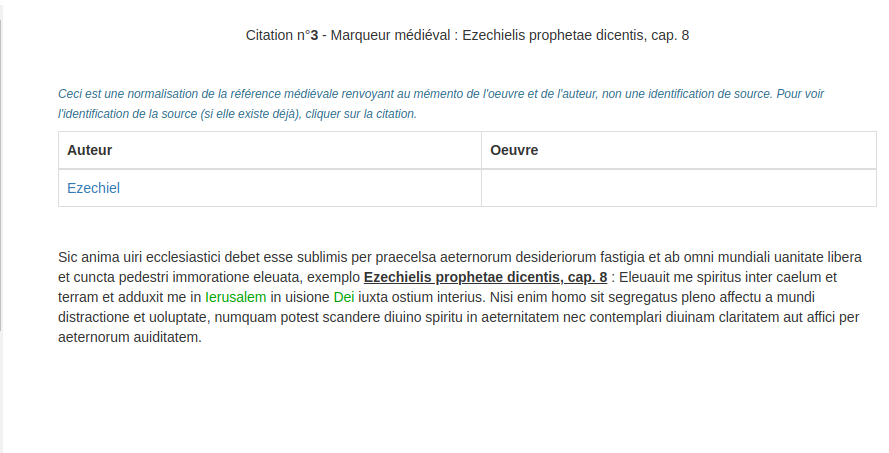
\includegraphics[width=0.6\linewidth]{images/mentionjerusalemsourcencyme.png}}
		\caption{Mention de Jérusalem dans SourcEncyMe}
	\end{figure}
	
\end{itemize}

Parmi les options de lien disponibles, j'ai décidé de me concentrer principalement sur les données. Cette décision repose sur plusieurs considérations : c’était un des objectifs principaux définis dans le livret de stage, et les utilisateurs s'intéressent principalement aux données, cherchant avant tout à accéder aux résumés de ThEMA et aux textes édités dans SourcEncyMe. Les \index{Mementos}mementos et les mots-clés, bien que facilitant les recherches thématiques, sont secondaires par rapport aux données essentielles pour la recherche historique. De plus, une \index{Encyclopédies}encyclopédie testée avait déjà fait l’objet d’un repérage préalable d’\textit{exempla} par une autre chercheuse de l’IRHT, Mara Calloni, et l’indexation des \index{Encyclopédies}encyclopédies dans ThEMA a facilité ce travail. 

En ce qui concerne les mots-clés, les noms de lieux et de personnes, le travail aurait été plus complexe, car SourcEncyMe n'a effectué qu'un repérage partiel à ce niveau dans les textes, contrairement à ThEMA. Quant aux liens vers les \index{Mementos}mementos, ils n'étaient pas prioritaires par rapport aux liens entre les textes, même s'ils auraient pu être établis assez facilement.


\section{Intégration des liens XML dans les bases de données}
Les textes des deux bases de données sont stockés dans des fichiers XML, ce qui a nécessité une réflexion sur l'insertion des liens et la recherche d'informations permettant de créer des liens. La gestion de ces liens a varié en fonction des spécificités de chaque base.

\subsection{Recherche des emplacements et des informations dans les XML pour la création des liens dans ThEMA}
Pour ThEMA, l'intégration des liens a été relativement simple. Les fichiers XML, un par \textit{exemplum}, comportaient déjà des balises spécifiques pour les liens, comme illustré dans l'exemple suivant : \\

\begin{lstlisting}[breaklines=true]
	<sourceDesc>
		<list type="source_details">
			<item type="source_text">
				<p/>
			</item>
			<item type="sources">
				<p/>
			</item>
			<item type="exemplum_context">
				<p>Feria quarta primae hebdomadae. Sermo I.</p>
			</item>
			<item type="commentary">
				<p/>
			</item>
			<item type="allegory">y</item>
		</list>
		<listBibl>
			<bibl type="manuscripts-editions" corresp="Z-IU7WR86C" n="t. I, p. 66-67"/>
		</listBibl>
		<list type="links">
			<item type="link" corresp="http://sermones.net/thesaurus/document.php?id=jvor_210">Sermones.net</item>
		</list>
		<list type="linked_exempla"/>
	</sourceDesc>
\end{lstlisting} 

\

\begin{figure}[H]
	\centering
	\fbox{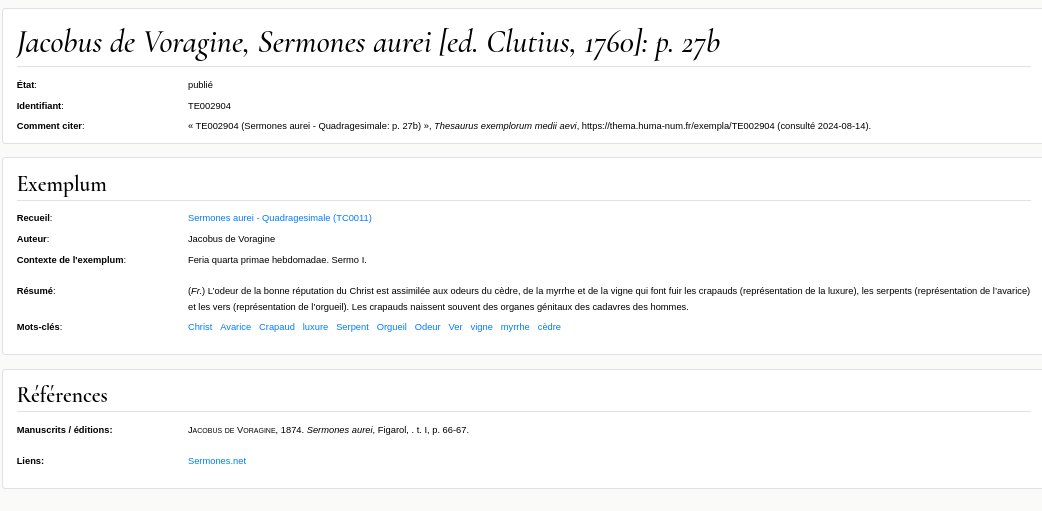
\includegraphics[width=0.8\linewidth]{images/exemplumaveclienthema.png}}
	\caption{Localisation du lien dans ThEMA}
\end{figure}

Les références aux \index{Encyclopédies}encyclopédies dans ThEMA se trouvent dans les champs « sources » et « textes apparentés ». Pour les récupérer, il faut naviguer dans les balises suivantes : <sourceDesc>, puis <list>, puis <item> avec l'attribut type="source", et enfin <p>. De même, pour les textes apparentés, il faut se rendre dans <sourceDesc>, puis <listBibl>, et enfin <bibl type="related\_texts"/>. \\

\

\begin{lstlisting}[breaklines=true]
	<sourceDesc>
		<list type="source_details">
			<item type="source_text">
				<p/>
			</item>
			<item type="sources">
				<p>Vincent de Beauvais, Speculum historiale, 13.50, dans Speculum quadruplex, vol. 4, 522a.</p>
			</item>
		<list>
	<sourceDesc>	
\end{lstlisting} 

\

\begin{lstlisting}[breaklines=true]
	</sourceDesc>
		<listBibl>
			<bibl type="related_texts" corresp="Z-E46747N6" n="p. 584"/>
			<bibl type="tubach" corresp="Z-WLZ7CBVC" n="TUB951"/>
		</listBibl>
		<list type="links"/>
		<list type="linked_exempla"/>
	</sourceDesc>
\end{lstlisting} 

\

\begin{figure}[H]
	\centering
	\fbox{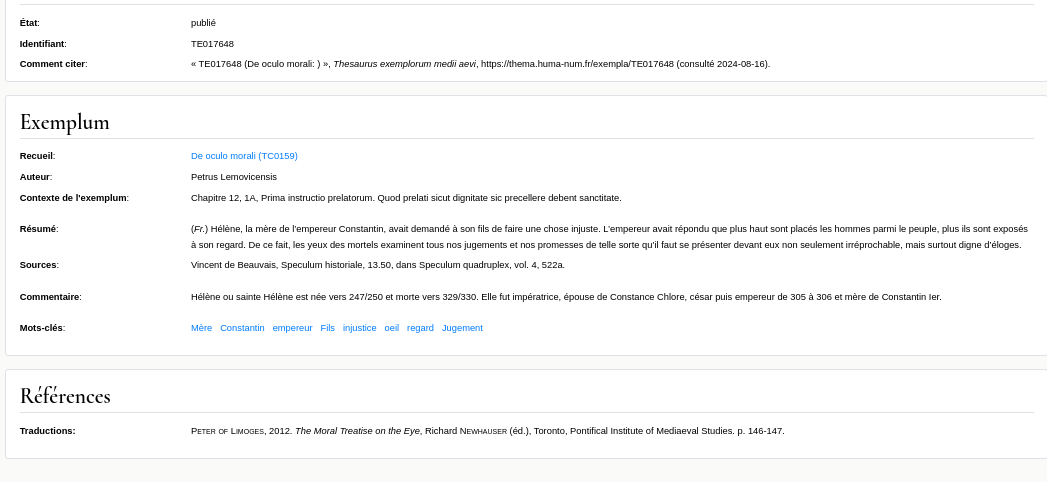
\includegraphics[width=0.8\linewidth]{images/vincentbeauvaisthema.png}}
	\caption{Champ source dans ThEMA}
\end{figure}

\subsection{Placement des liens et des visualisation des \textit{exempla} dans les XML de SourcEncyMe}

En revanche, dans SourcEncyMe, il n'existe pas de balises spécifiques pour intégrer les liens vers ThEMA. Chaque \index{Encyclopédies}encyclopédie est intégrée dans un fichier \index{XML}XML unique, comme montré dans l'annexe E. Initialement, j'avais envisagé d'ajouter de nouvelles balises <ref> avec un attribut spécifique pour les liens, en conformité avec les Tei Guidelines\footcite{17LinkingSegmentation}. Ce lien aurait été intégré dans la balise <cit> du XML, car dans SourcEncyMe, chaque citation d'un auteur est placée dans une balise <cit>. Voici la structure envisagée : \\

\begin{lstlisting}[breaklines=true]
<cit xml:id="cit_idp103803440">
	<bibl>
		<author ref="#gregorius_nazianzenus">Gregorius Nazianzenus</author>
	</bibl>
	<quote>Et hinc est quod venerabilis doctor<seg type="marqueur">Gregorius Nazianzenus</seg>cuius (testante<seg type="marqueur">Hieronymus</seg>) tanta auctoritas fuit&#160;: ut nullus unquam eius dictis calumniam inferre presumpserit&#160;: Immo insuper (ut testatur<seg type="marqueur">Rufinus</seg>) tanta fuit eius auctoritas apus ecclesias Christi, ut esse putaretur hereticus qui illi fuisset ausus in aliquo contraire. Hic itaque doctor hanc sibi consuetudinem fecerat, ut quicquid eius occurreret oculis de rebus exterioribus, interioribus anime moribus adaptaret&#160;: Sic enim refert ipse de se in suo apologetico, dicens&#160;: Mos mihi est ad meipsum singula queque revocare, precipue si quies mihi, sit, et silentium si vacet, animi moribus adaptare quod videtur in oculis. Unde et oculorum visio est mihi mentis eruditio. Huius igitur exemplum laudabile sequi oportet, si abundare volunt copia exemplorum. Que copia illis si affuerit, precipue de rebus extrinsecis que nobis sunt in aperto, et etiam de mirandis operibus que continue natura producit, vel adinvenit humana industria&#160;: non eos tantum apud curiosos auditores faciet gratiosos, quos mira nature opera vel humane inventionis studia narrata et patefacta delectant, sed etiam apud vulgus et simplices fructuosos et acceptos constituet, dum per exempla ad sensum spiritualia et subtilia declarabunt.
	</quote>
</cit>
\end{lstlisting}

Cependant, en plus de ce changement dans le XML, il aurait également fallu modifier le code de la base de données pour faire apparaître les liens. Cela aurait aussi posé problème car cela modifiait la structure globale du XML. Par conséquent, avec l’ingénieur de recherche Emmanuelle Khury, nous avons décidé d’intégrer les liens dans une balise préexistante pour éviter tout changement dans le XML. Nous avons choisi de placer le lien dans l’attribut correspondant de la balise <ref> qui se trouve dans la balise <bibl>. Cette dernière est utilisée dans SourcEncyMe pour indiquer une œuvre, comme vous pouvez le voir ici : \\

\begin{lstlisting}[breaklines=true]
	<cit n="2" xml:id="cit_id394697881596">
		<bibl>
			<ref target="#historiarum_adversum_paganos_orosii_libri_vii" type="oeuvre">Historiarum adversum paganos Orosii libri VII</ref>
			<author ref="#orosius_paulus">Orosius Paulus</author>
		</bibl>
		<bibl>
			<ref cert="low" corresp="https://thema.huma-num.fr/exempla/TE022184" target="#exemplum">Exemplum</ref>
		</bibl>
		<quote>
			<seg type="marqueur">Orosius de hormesta mundi libro primo</seg>Extant adhuc certissima monumenta gestorum. Nam tractus curruum et orbite rotarum, non solum in littore, sed etiam in profundo, nunc quousque visus admittitur pervidentur. Et si forte ad tempus casu vel curiositate conturbatur, mox divinitus in pristinam faciem ventis, fluctibusque reparantur, ut quisquis non docetur timore dei vel probate religionis studio, ita eius transacte ultionis terreatur <seg type="marqueur">exemplo.</seg>
		</quote>
	</cit>
\end{lstlisting}

\

De plus, un attribut cert="low" a été ajouté pour indiquer un faible taux de certitude, étant donné que l'ajout des liens a été automatisé\footnote{Il s'agissait de bien différencier les repérages faits de manière manuelle et ceux réalisés de manière automatique pour les chercheurs, dans un souci de transparence. Cette idée a été proposée par Emmanuelle Kuhry et Isabelle Draelants.}. De plus, si plusieurs liens sont présents, ils seront séparés par des espaces dans le même attribut corresp. Le lien sera visible car ce qui est inclus dans les balises <bibl> des balises <cit> est déjà affiché par le code de la base de données : \\

\begin{figure}[H]
	\centering
	\fbox{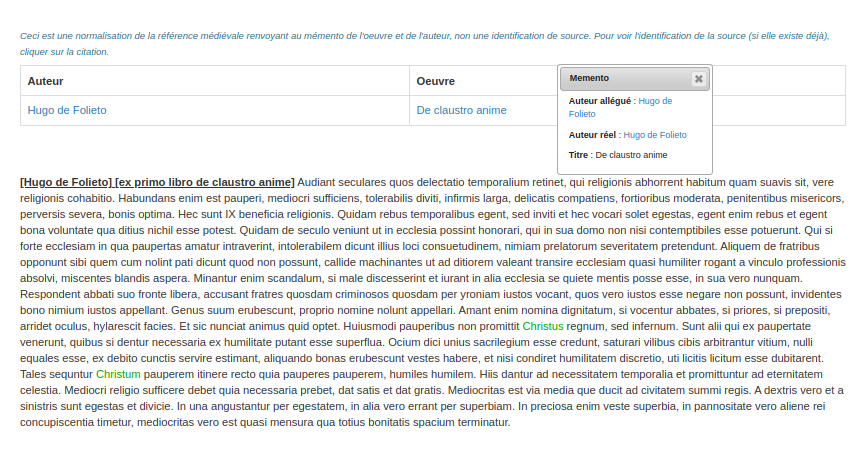
\includegraphics[width=0.7\linewidth]{images/affichagesourcencymeoeuvre.png}}
	\caption{Affichage de l'oeuvre dans SourcEncyMe}
\end{figure}

Enfin, pour indiquer la présence d'un \textit{exemplum} dans le texte, des marqueurs sont utilisés pour surligner le début du récit exemplaire ou son introduction (voir le code au-dessus). Bien que ces marqueurs soient normalement utilisés pour signaler le début d'une citation, ils ont été détournés de leur fonction initiale pour les \index{Récits exemplaires}récits exemplaires\footcite{SourcEncyMe}. Cependant, ces marqueurs ne sont présents que lorsque l'\textit{exemplum} est explicitement introduit, ce qui n'est pas toujours le cas.